%!TEX root = ../physical-olympics-2.tex
\chapter{量子论}

我们用选自\emph{费曼}(R. Feynman)先生的物理学讲义的开篇金句来作为本章与下一章近代物理内容的开头:
\begin{quote}
Each piece, or part, of the whole of nature is always merely an approximation to the complete truth. Therefore, things must be learned only to be unlearned again or, more likely, to be corrected. The test of all knowledge is \emph{experiment}. Experiment is the sole judge of scientific ``truth''.
\end{quote}

的确,\,量子理论以其不直观而被近代早期物理学家们所疑惑,\,这其中不乏一些赫赫有名的大师.\,直到现在也有很多基础的问题是没有被深刻地理解的:\,电子的本性与内部结构,\,基本粒子的类别与参数,\,对量子非定域性与测量的理解...\,所以在关于可能会造成问题的领域的学习时,\,需要先明白实验上的事实,\,从中理解理论建立的必要性.


\section{黑体辐射}

对于\emph{热辐射}(thermal radiation)的讨论是何时进入物理研究的视野的呢?\,可以肯定的是人类认识到热辐射现象非常的早:\,光芒万丈的太阳,\,烧红的木炭与金属都是典型的热辐射的情形.\,但人们掌握足够的方法去测量它则也是要到19世纪后半期了.\,热辐射势必涉及到电磁场与电荷的相互作用.\,而且深入到原子尺度,\,实际上就是电磁波的发射与吸收.\,对于电磁波的发射,\,我们在电磁学中粗略讲过,\,只要有加速运动的电荷就会导致电磁辐射.\,之后小节我们将认识到微观电荷不能用``加速''来描述,\,其状态其实是量子态,\,处于激发态才会自发向基态去跃迁放出电磁辐射.\,而对于电磁波的吸收,\,则在光学中我们简要介绍过洛伦兹电子论中的处理方法.\,

\begin{wrapfigure}[9]{o}[0pt]{7cm}
\centering
\vspace{-15pt}
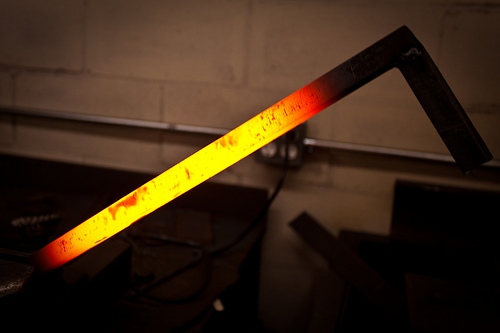
\includegraphics[width=7cm]{image/19-1-1.jpg}
\caption{热辐射}
\end{wrapfigure}
一个物体如果能够在任何温度下把照射到它上面的任何频率的光都全部吸收掉,\,那么这个物体就叫做\emph{黑体}(black body).\,虽然在现实生活中这样的物体并不存在,\,但石墨和碳黑往往被视作比较理想的黑体,\,尽管这样,\,黑体``看上去''也不总是``黑的''.\,著名生物学家查尔斯·达尔文的一个亲戚,\,陶瓷师,\,托马斯·玮致活在1792年注意到所有物体,\,不论化学构成,\,形状,\,尺寸,\,几乎都在相同的温度下烧红.\,黑体也不例外.\,作为这个实验现象研究的推广,\,1859年\emph{基尔霍夫}(G. Kirchhoff)利用热力学理论证明了著名的\emph{基尔霍夫定律}:\,即对于某角频率的光波,\,某温度下任意物体的辐射本领正比于吸收率:
\[e(\omega)=J(\omega,\,T)A(\omega)\]

其中,\,$e$为单位面积单位时间单位角频率间隔辐射的能量,\,而$A$为对该频率光的吸收率.\,$0<A<1$.\,除了吸收以外就是反射.\,物体较薄时还存在透射.\,不同物体在相同的$T,\,\omega$下可以有不同的$A,\,e$,\,但是其比值$J$却是一个\emph{普适}(universal)的函数.\,即与物体本身没有关系.\,而黑体的定义为$A(\omega)$恒等于$1$.\,也就是说明了黑体的辐射本领:
\[e(\omega)=J(\omega,\,T)\]

之后人们的任务就非常清晰了:\,测出不同$T$下的函数$J(\omega,\,T)$.\,而这个过程大致可以分为三个阶段:

1.\,挖掘出$J(\omega,\,T)$的整体特征.

2.\,实验测量$J(\omega,\,T)$的曲线与提出可能的理论模型.

3.\,最终确定$J(\omega,\,T)$的函数形式与理论解释.

\[J(\omega,\,T)=\frac{1}{4}u(\omega,\,T)c\]

\[u(\omega,\,T)=\frac{C_1\omega^3}{e^{C_2\omega/kT}-1}\]


\section{光粒子性}

\section{玻尔原子}

\section{电子波动性}

\section{物质波与波函数}

